\section{Objective 1: \texttt{mpbenchmark}}

Results from the proposed solution collected from desktop(\texttt{x86} processor) are shown below, they are presented in the legend ``C++" and ``C++(SIMD Optimised)". A benchmark plot along with a speedup plot are shown in figures ~\ref{fig:mpbenchmark_desktop_plot} and ~\ref{fig:mpbenchmark_desktop_speedup_plot} respectively. Full system specifications of the desktop(\texttt{x86}) along with the Raspberry Pi processors can be found in the appendix.

\begin{figure}[htbp] % Positioning preference: here, top, bottom, page
	\centering
	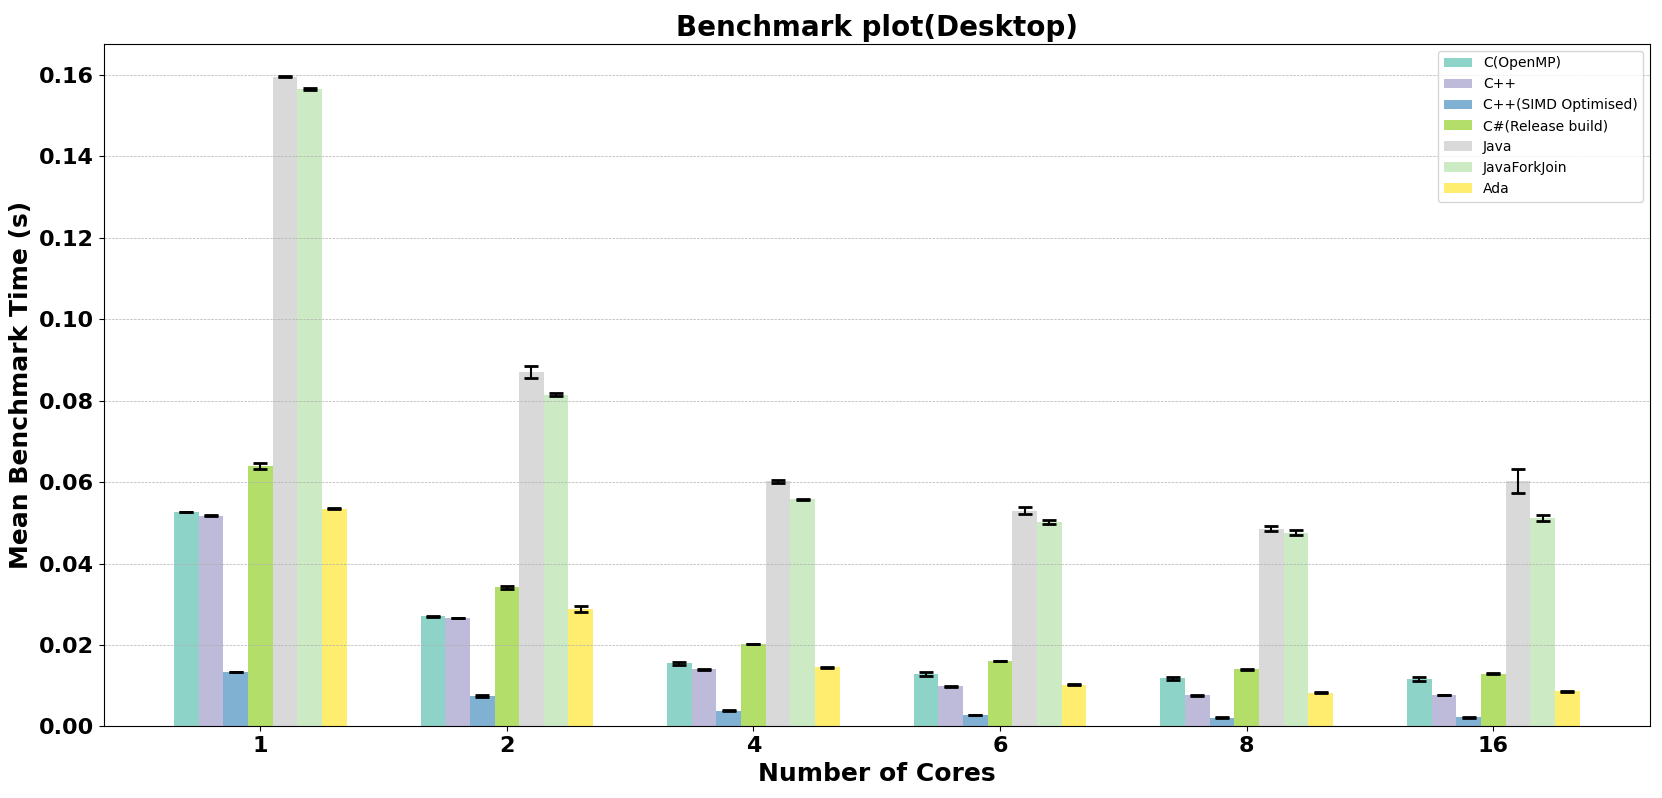
\includegraphics[width=1\textwidth, height=20cm]{~/Documents/Part_D_Modules/Individual_Project/Individual_report/figures/mpbenchmark_desktop.png} % Adjust the path and width as needed
	\caption{Mean benchmark plot of \texttt{mpbenchmark} collected from \texttt{x86} processor in seconds. The error bars represent 95\% confidence interval. (Lower is better).}
	\label{fig:mpbenchmark_desktop_plot} % Use this label to reference the figure
\end{figure}


\begin{figure}[htbp] % Positioning preference: here, top, bottom, page
	\centering
	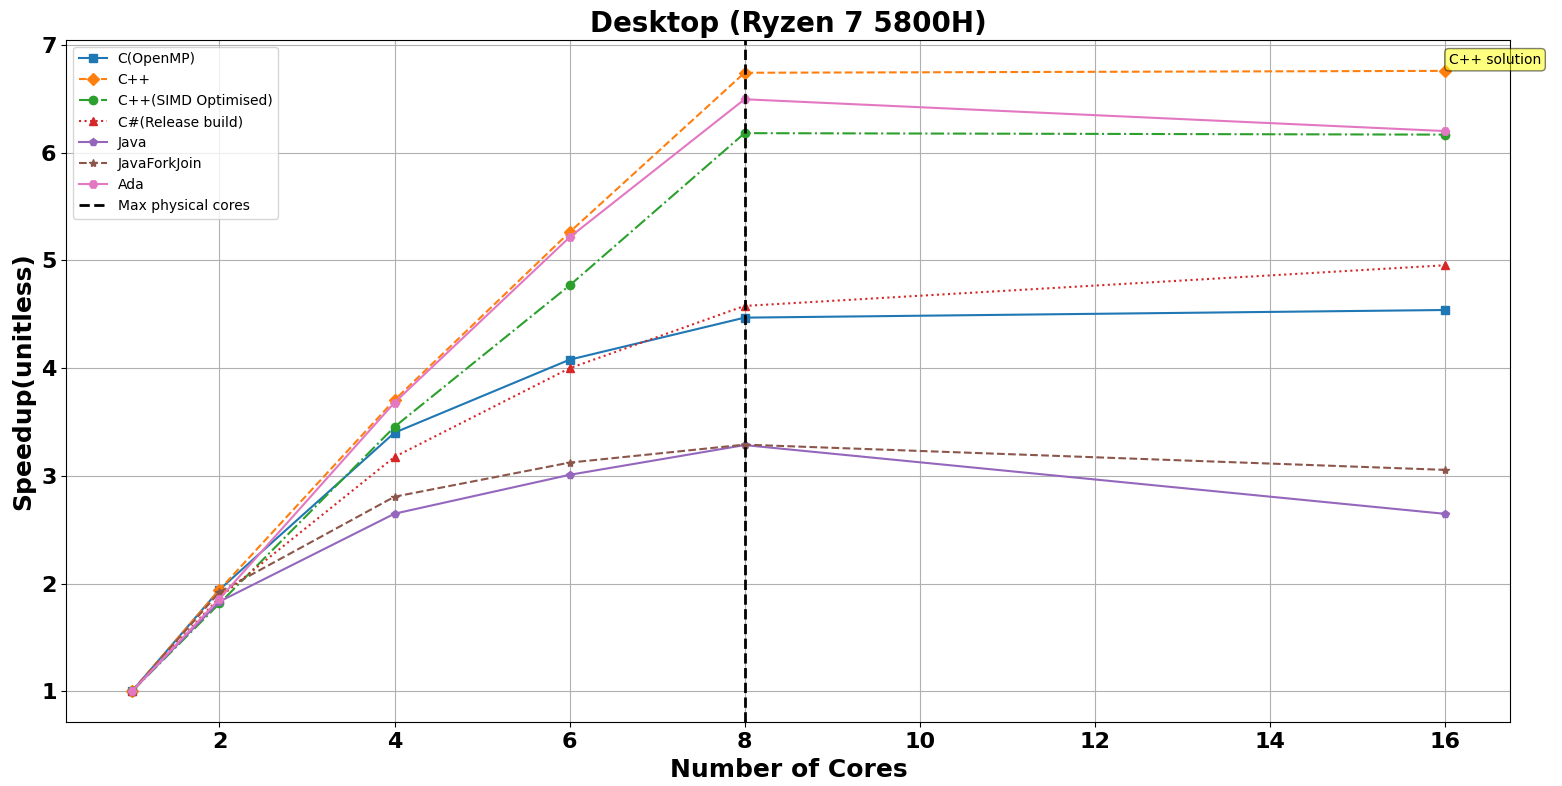
\includegraphics[width=1\textwidth, height=20cm]{~/Documents/Part_D_Modules/Individual_Project/Individual_report/figures/mpbenchmark_desktop_speedup.png} % Adjust the path and width as needed
	\caption{Speedup plot collected from \texttt{x86} processor. The vertical black line shows the maximum physical cores of the processor. (Higher is better).}
	\label{fig:mpbenchmark_desktop_speedup_plot} % Use this label to reference the figure
\end{figure}

On desktop(\texttt{x86}) processor, \texttt{AVX2} instructions were used to implement SIMD intrinsics therefore we compare the decimal precision with the original unoptimised SIMD code, see table ~\ref{tab:c++_avx2_pi}.

\begin{table}[htbp]
	\centering
	\begin{tabular}{|c|c|c|}
		\hline
		\textbf{Programming language/configuration} & \textbf{Decimal value of $\pi$} & \textbf{Mean run time using maximum threads(s)} \\ \hline
		\texttt{C++}             & 3.1415926535897643 &  0.007659 \\ \hline
		\texttt{C++/AVX2}   & 3.1415926535899033 &  0.002173  \\ \hline
		\texttt{C}                 & 3.1415926535897643 & 0.011577 \\ \hline
		\texttt{Ada}             & 3.1415926535897643 &  0.008623\\ \hline
	\end{tabular}
	\label{tab:c++_avx2_pi}
	\caption{Comparing the decimal precision of the \texttt{AVX2} enhanced solution with the original.}
\end{table}

% Talk about C++ solution outperforming the original in both run times and speedup 
% C++ SIMD enhanced outperformed even more with a lower speedup.
% Talk about SMT's benefits if any
% Discuss AVX2's decimal precision

The proposed \texttt{C++} solution outperformed the original implementations in \texttt{C} and \texttt{Ada} by over 11\%, marking a significant reduction in runtime. Additionally, it achieved a higher speed-up compared to the \texttt{Ada} solution, as illustrated in figure~\ref{fig:mpbenchmark_desktop_speedup_plot}. The SIMD-enhanced solution achieved a remarkable runtime reduction of over 70\%, significantly outperforming all other solutions. However, this version did not show as large a speedup when run with an increased number of threads, which is not surprising given the already low runtime with a single thread. Moreover, the \texttt{AVX2}-enhanced code demonstrated decimal precision up to 12 decimal places, with discrepancies appearing from the 13th decimal place onwards, as shown in table~\ref{tab:c++_avx2_pi}. This suggests a slight consideration that using \texttt{AVX2} instructions might lead to reduced precision for calculations requiring high decimal accuracy. However, the reduction in decimal precision has been minor, and its effects on the application have been largely inconsequential. Given the dramatic improvement in performance with \texttt{AVX2} instructions, the minor loss of decimal precision seems negligible compared to the benefits. Both solutions have met their objectives, with the first achieving superior speed-up and the second providing insights into CPU performance when SIMD intrinsics are utilized.

Another noteworthy observation is the lack of performance gain when scaling from 8 to 16 cores. The processor used supports simultaneous multi-threading (SMT), commonly branded as ``Hyper-threading" for Intel CPUs, which is typical in modern \texttt{x86} processors. SMT theoretically allows each physical core to execute two threads, and an 8-core processor with SMT would appear to have 16 cores. However, the proposed solutions, along with other compiled languages like \texttt{C} and \texttt{Ada}, showed negligible performance gains by utilizing the virtual cores. \texttt{Java} experienced a slight performance degradation, while \texttt{C\#} was the only language to demonstrate a performance increase. Using the results from the \texttt{x86} processor, we can conclude that the additional cores provided by SMT did not enhance performance and, in some cases, even degraded it.

Results obtained from the latest Raspberry Pi 5 (\texttt{Cortex A-76} processor) are shown in figures ~\ref{fig:mpbenchmark_rpi5_plot} and ~\ref{fig:mpbenchmark_rpi5_speedup_plot}. The results obtained from the Raspberry Pi 4(\texttt{Cortex A-72} processor) are shown in figures ~\ref{fig:mpbenchmark_rpi4_plot} and ~\ref{fig:mpbenchmark_rpi4_speedup_plot}.

\begin{figure}[htbp] % Positioning preference: here, top, bottom, page
	\centering
	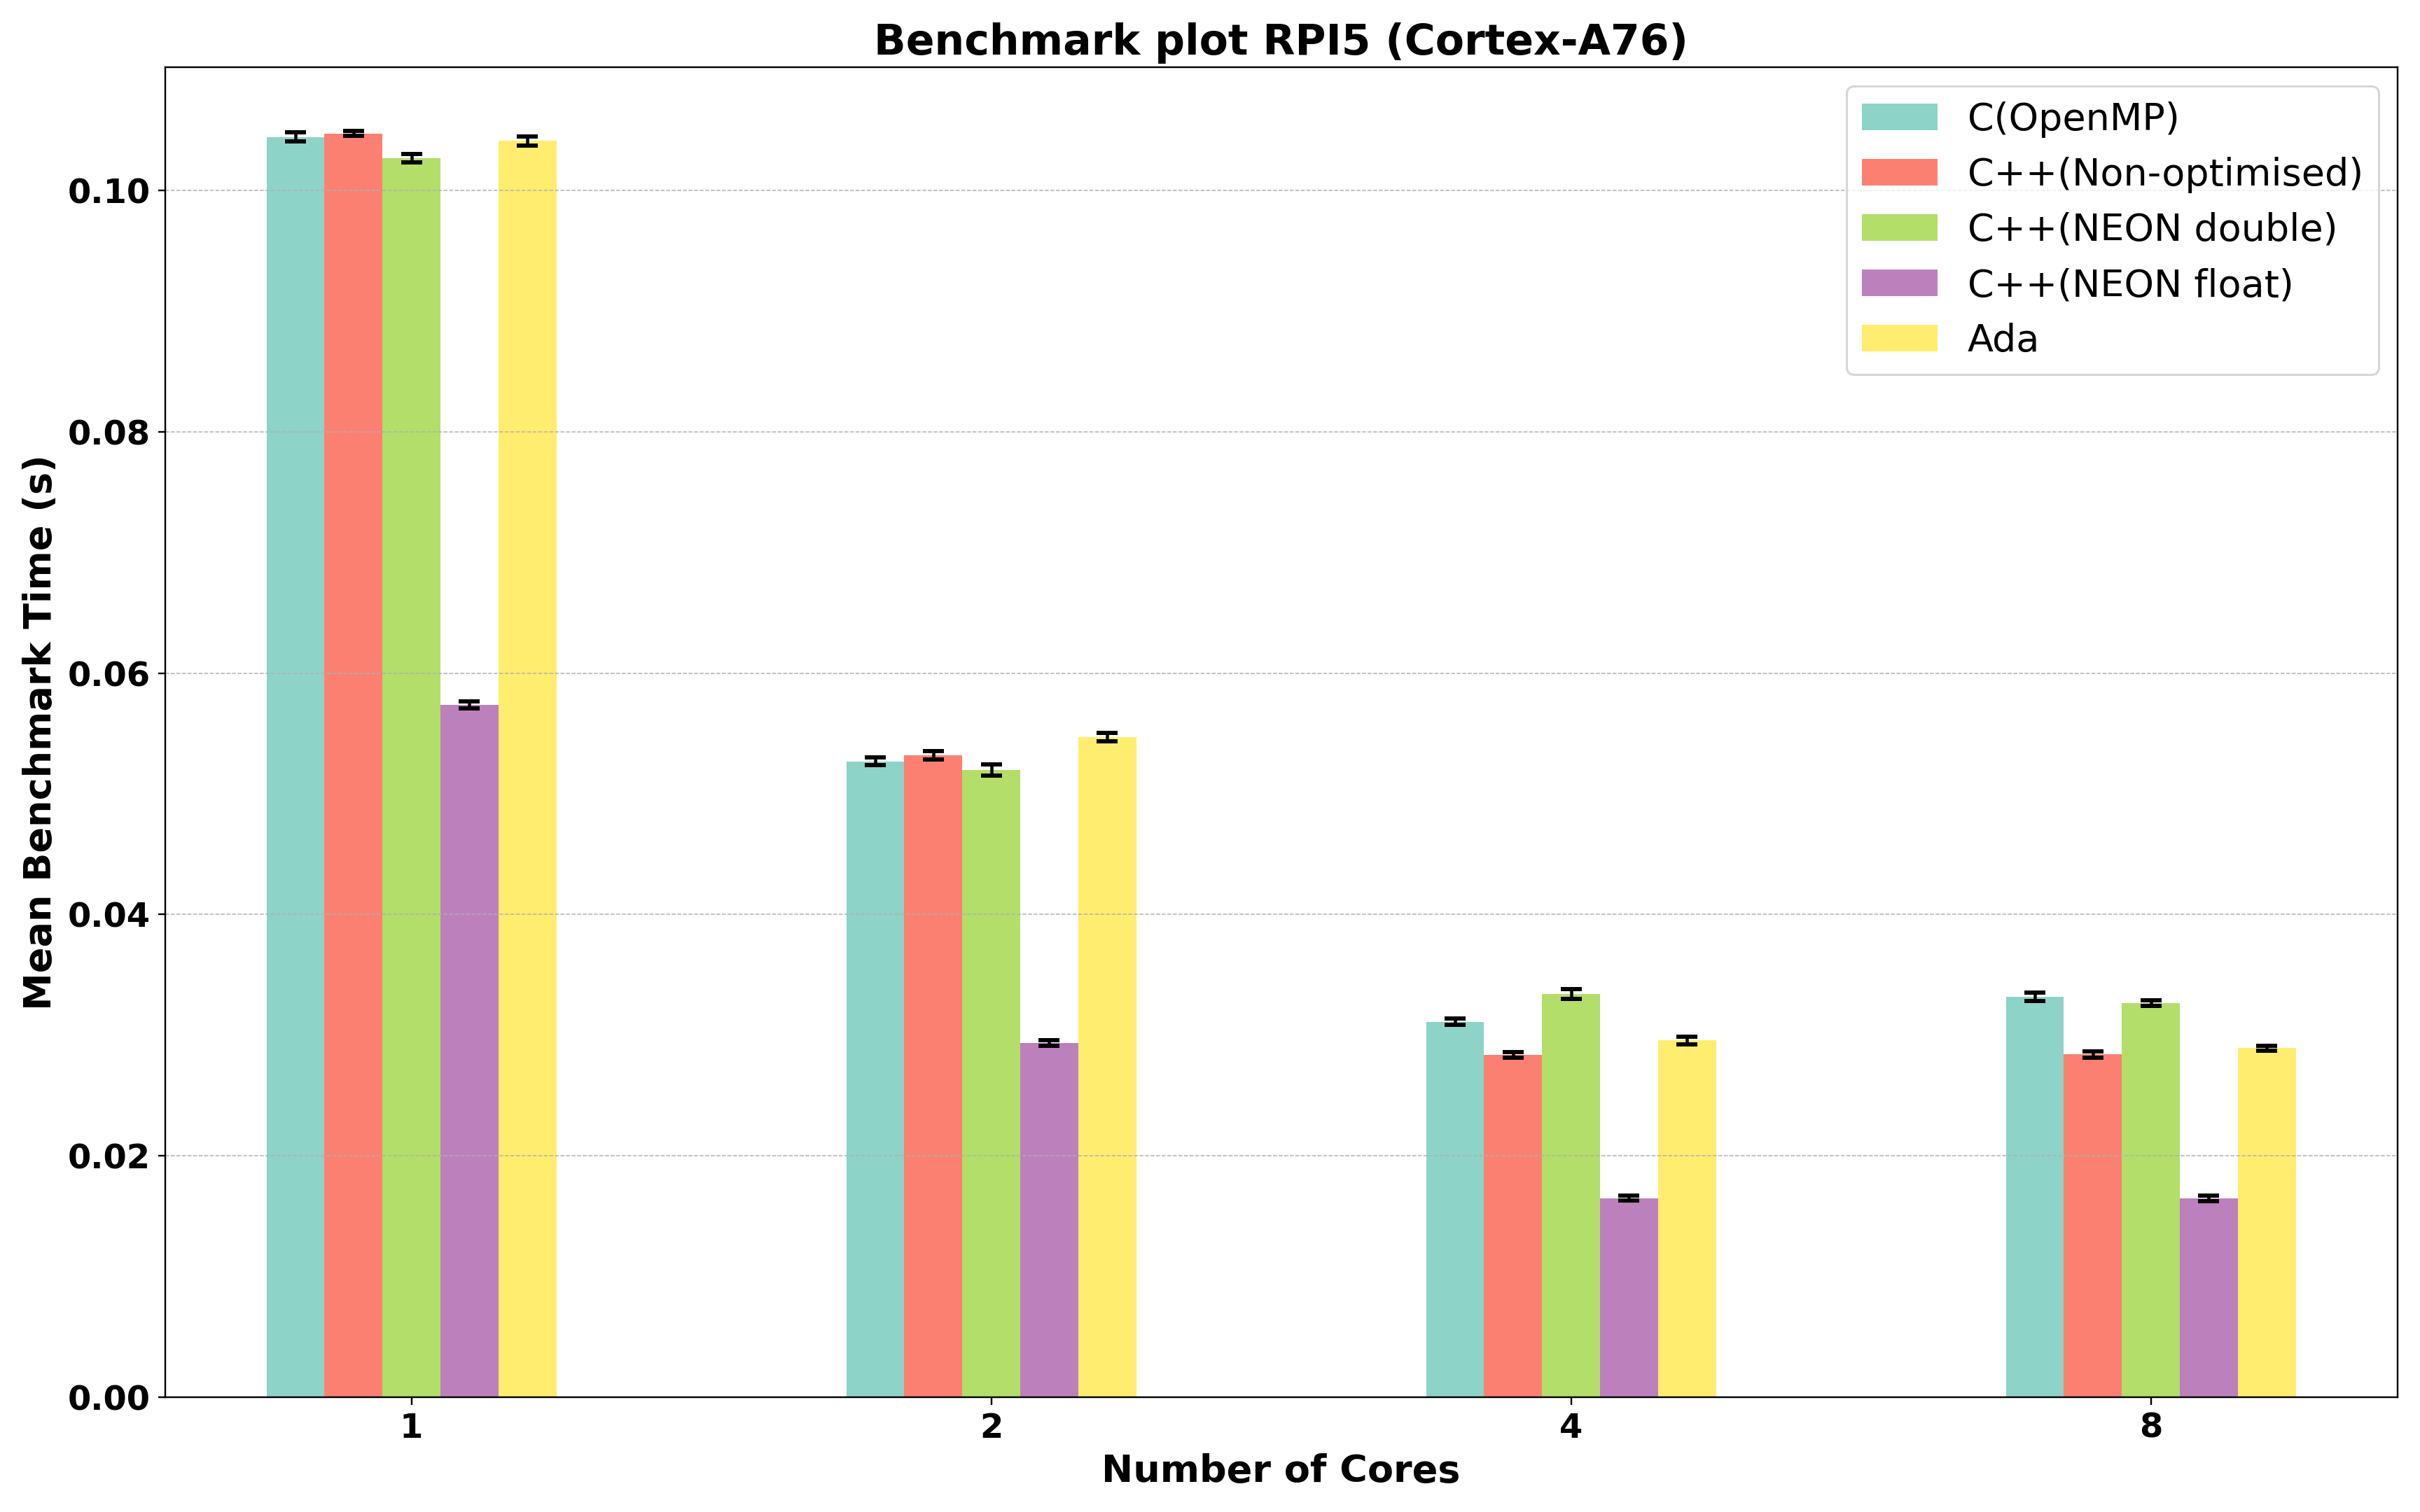
\includegraphics[width=1\textwidth, height=20cm]{~/Documents/Part_D_Modules/Individual_Project/Individual_report/figures/mpbenchmark_rpi5.png} % Adjust the path and width as needed
	\caption{Mean benchmark plot of results collected from Raspberry Pi 5(in seconds). The error bars represent 95\% confidence interval. (Lower is better).}
	\label{fig:mpbenchmark_rpi5_plot} % Use this label to reference the figure
\end{figure}

\begin{figure}[htbp] % Positioning preference: here, top, bottom, page
	\centering
	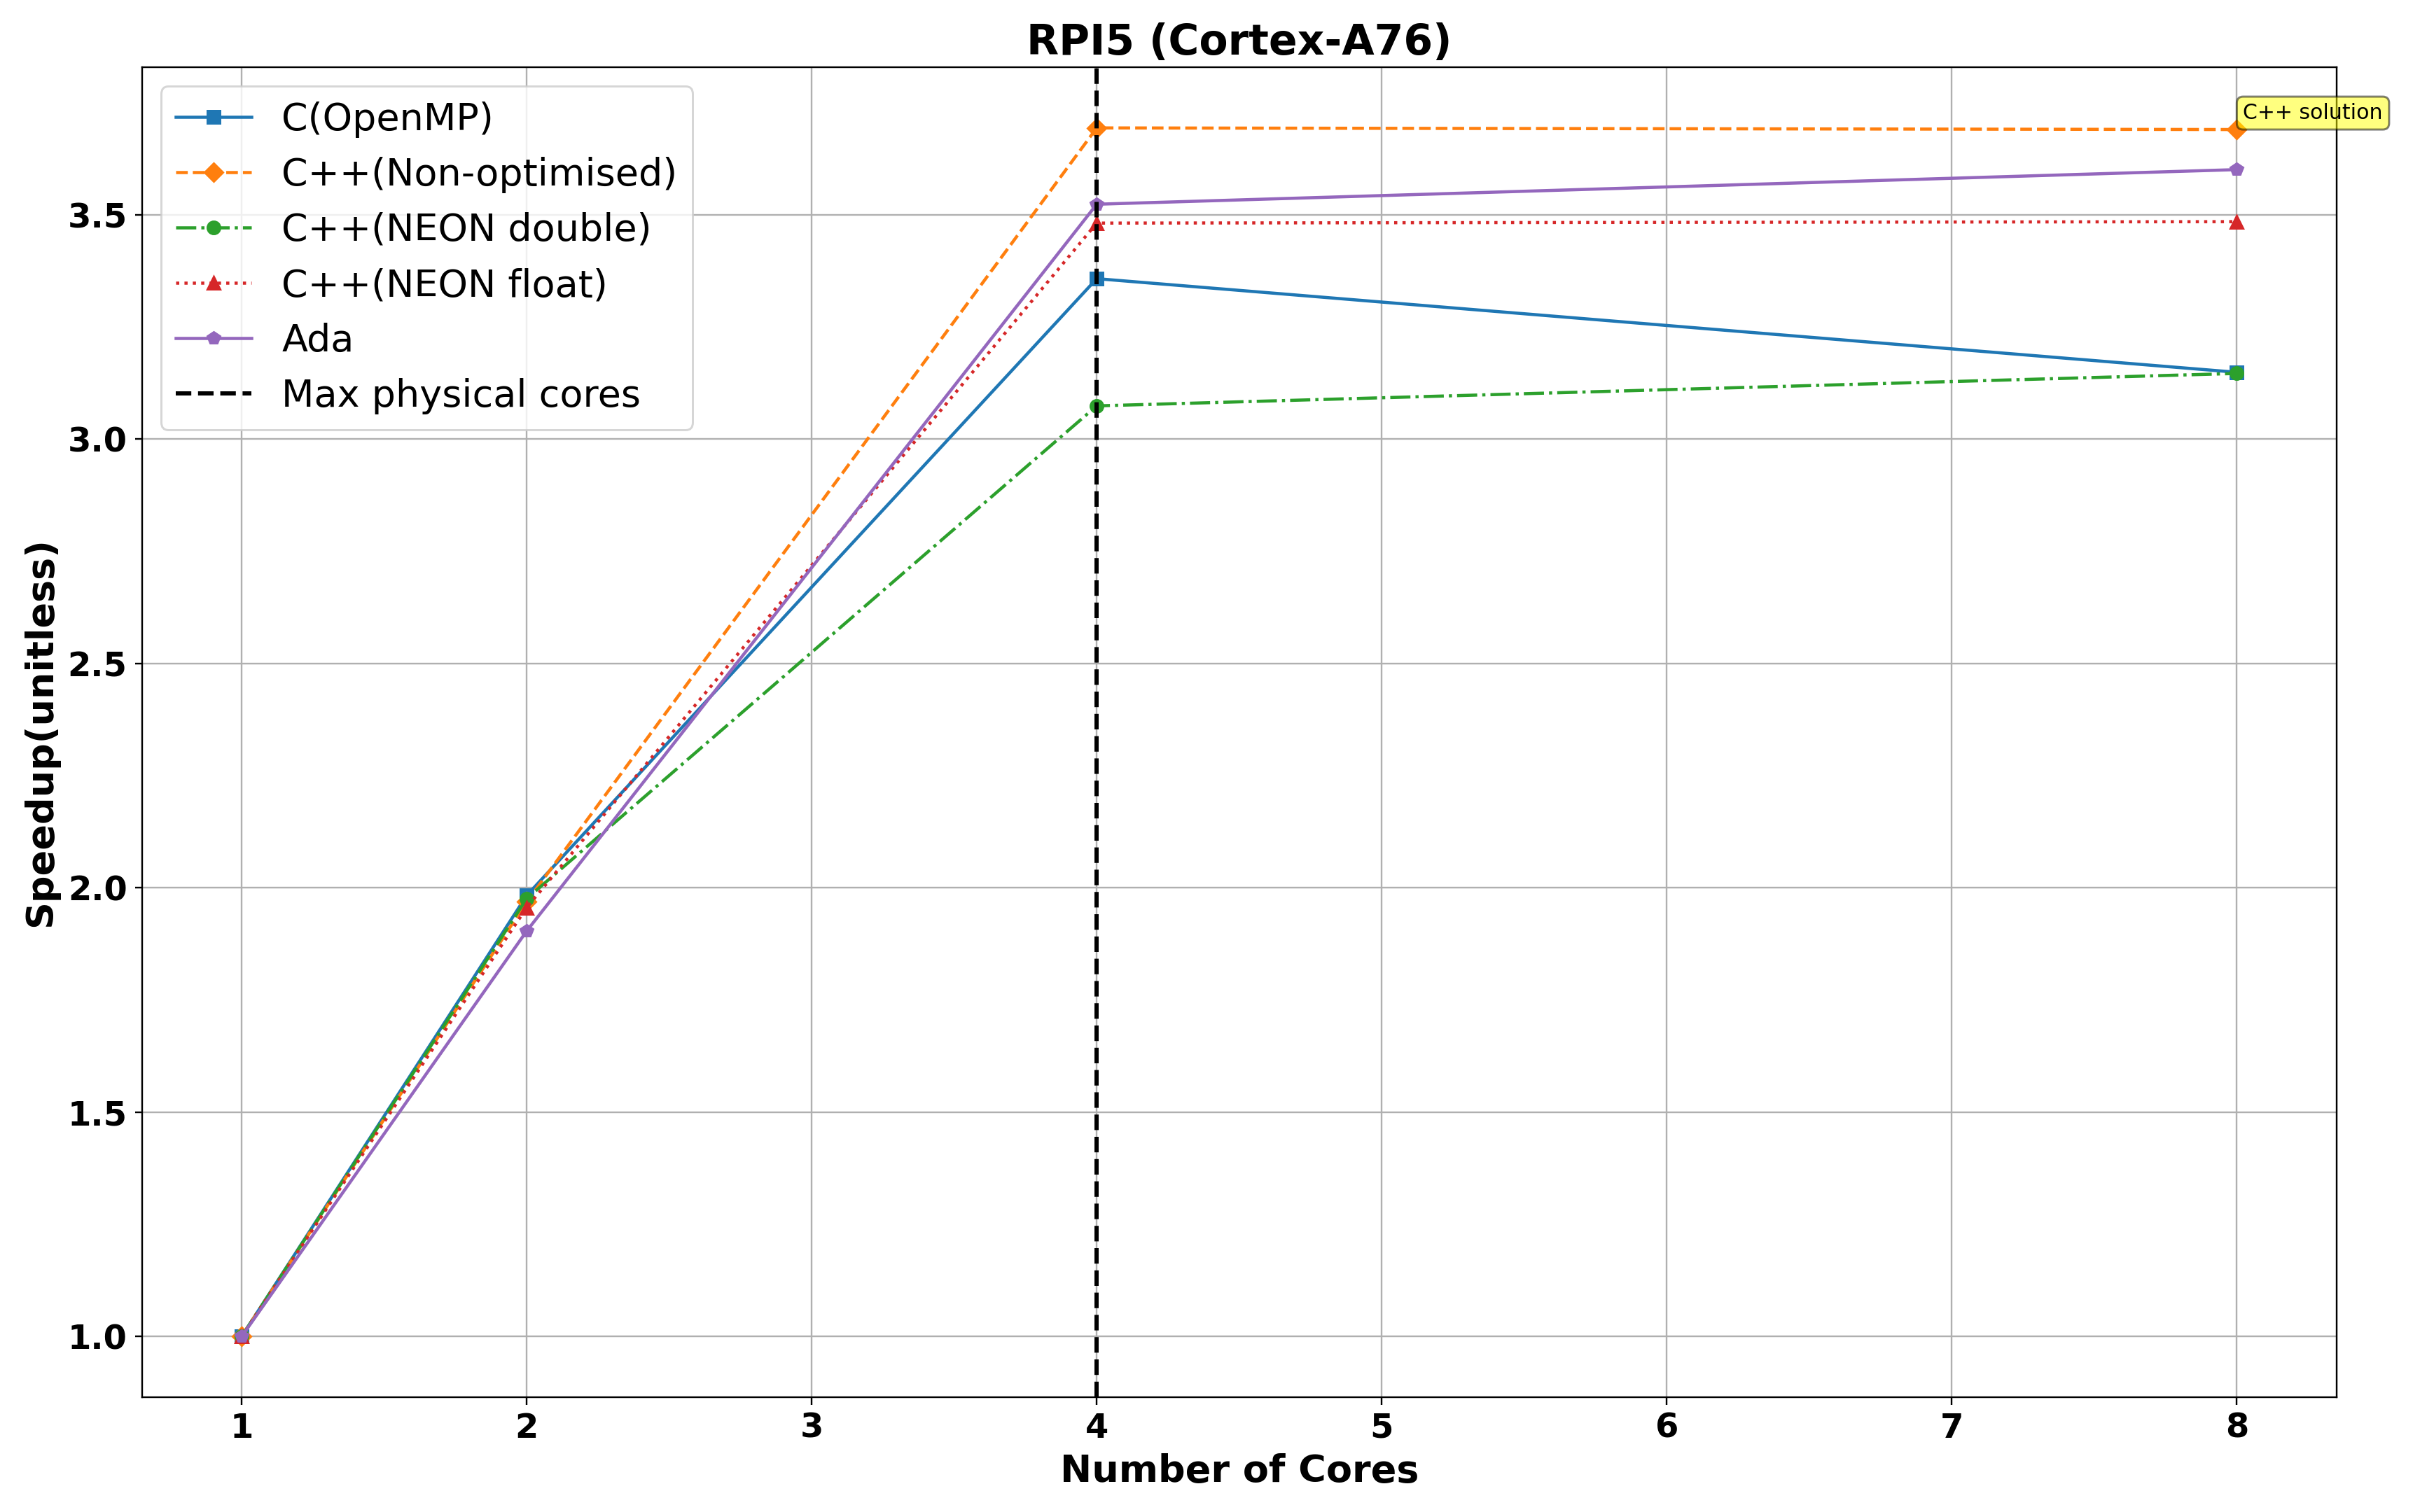
\includegraphics[width=1\textwidth, height=20cm]{~/Documents/Part_D_Modules/Individual_Project/Individual_report/figures/mpbenchmark_rpi5_speedup.png} % Adjust the path and width as needed
	\caption{Speedup plot collected from Raspberry Pi 5 processor. The vertical black line shows the maximum physical cores of the processor. (Higher is better).}
	\label{fig:mpbenchmark_rpi5_speedup_plot} % Use this label to reference the figure
\end{figure}

\begin{figure}[htbp] % Positioning preference: here, top, bottom, page
	\centering
	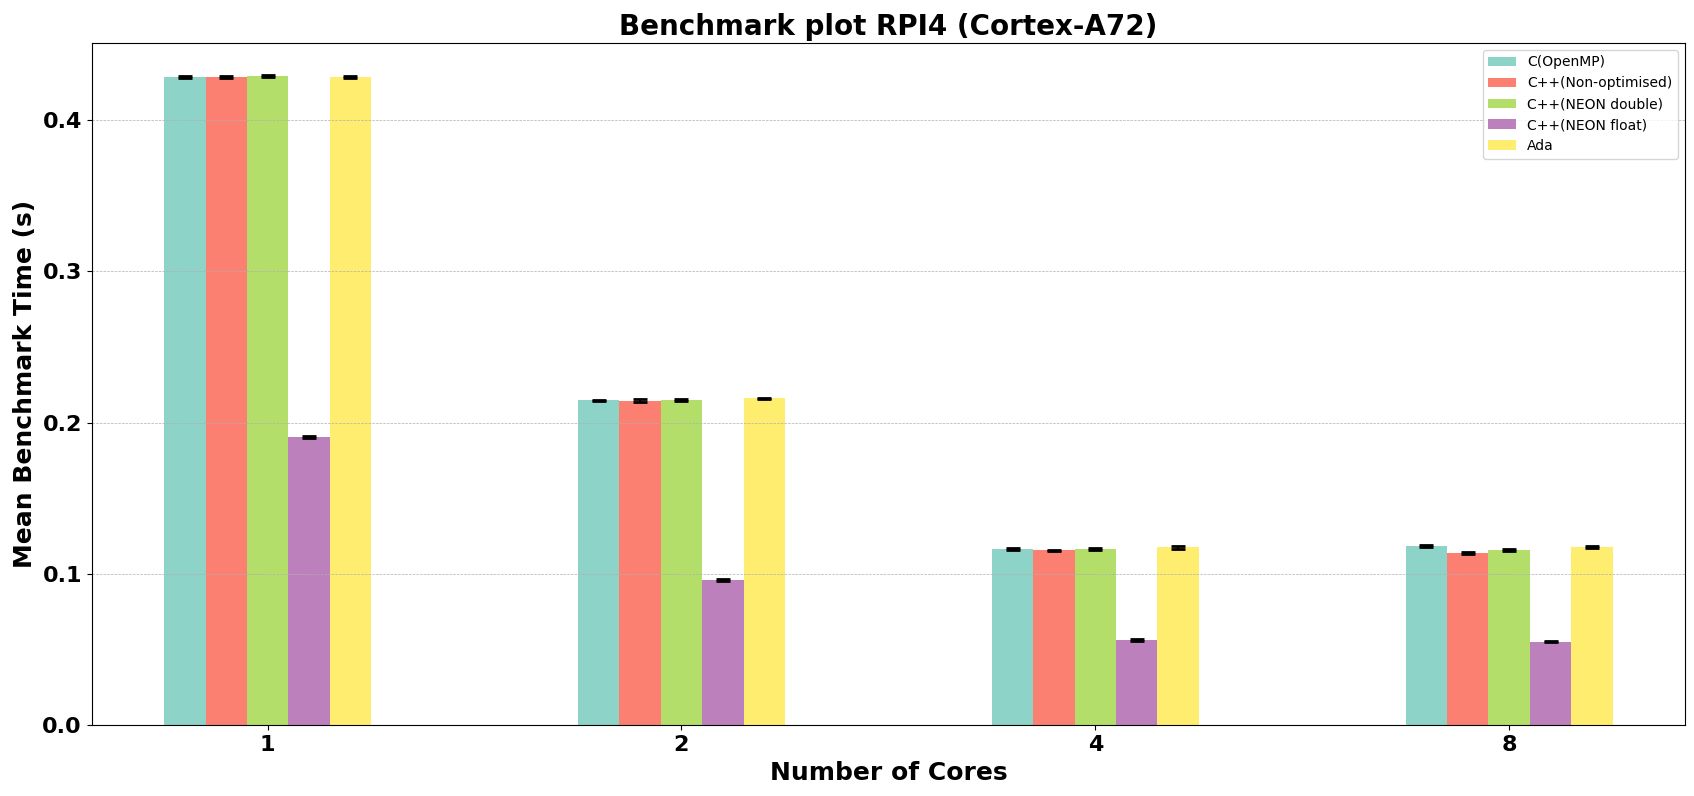
\includegraphics[width=1\textwidth, height=20cm]{~/Documents/Part_D_Modules/Individual_Project/Individual_report/figures/mpbenchmark_rpi4.png} % Adjust the path and width as needed
	\caption{Mean benchmark plot of results collected from Raspberry Pi 4(in seconds). The error bars represent 95\% confidence interval. (Lower is better).}
	\label{fig:mpbenchmark_rpi4_plot} % Use this label to reference the figure
\end{figure}

\begin{figure}[htbp] % Positioning preference: here, top, bottom, page
	\centering
	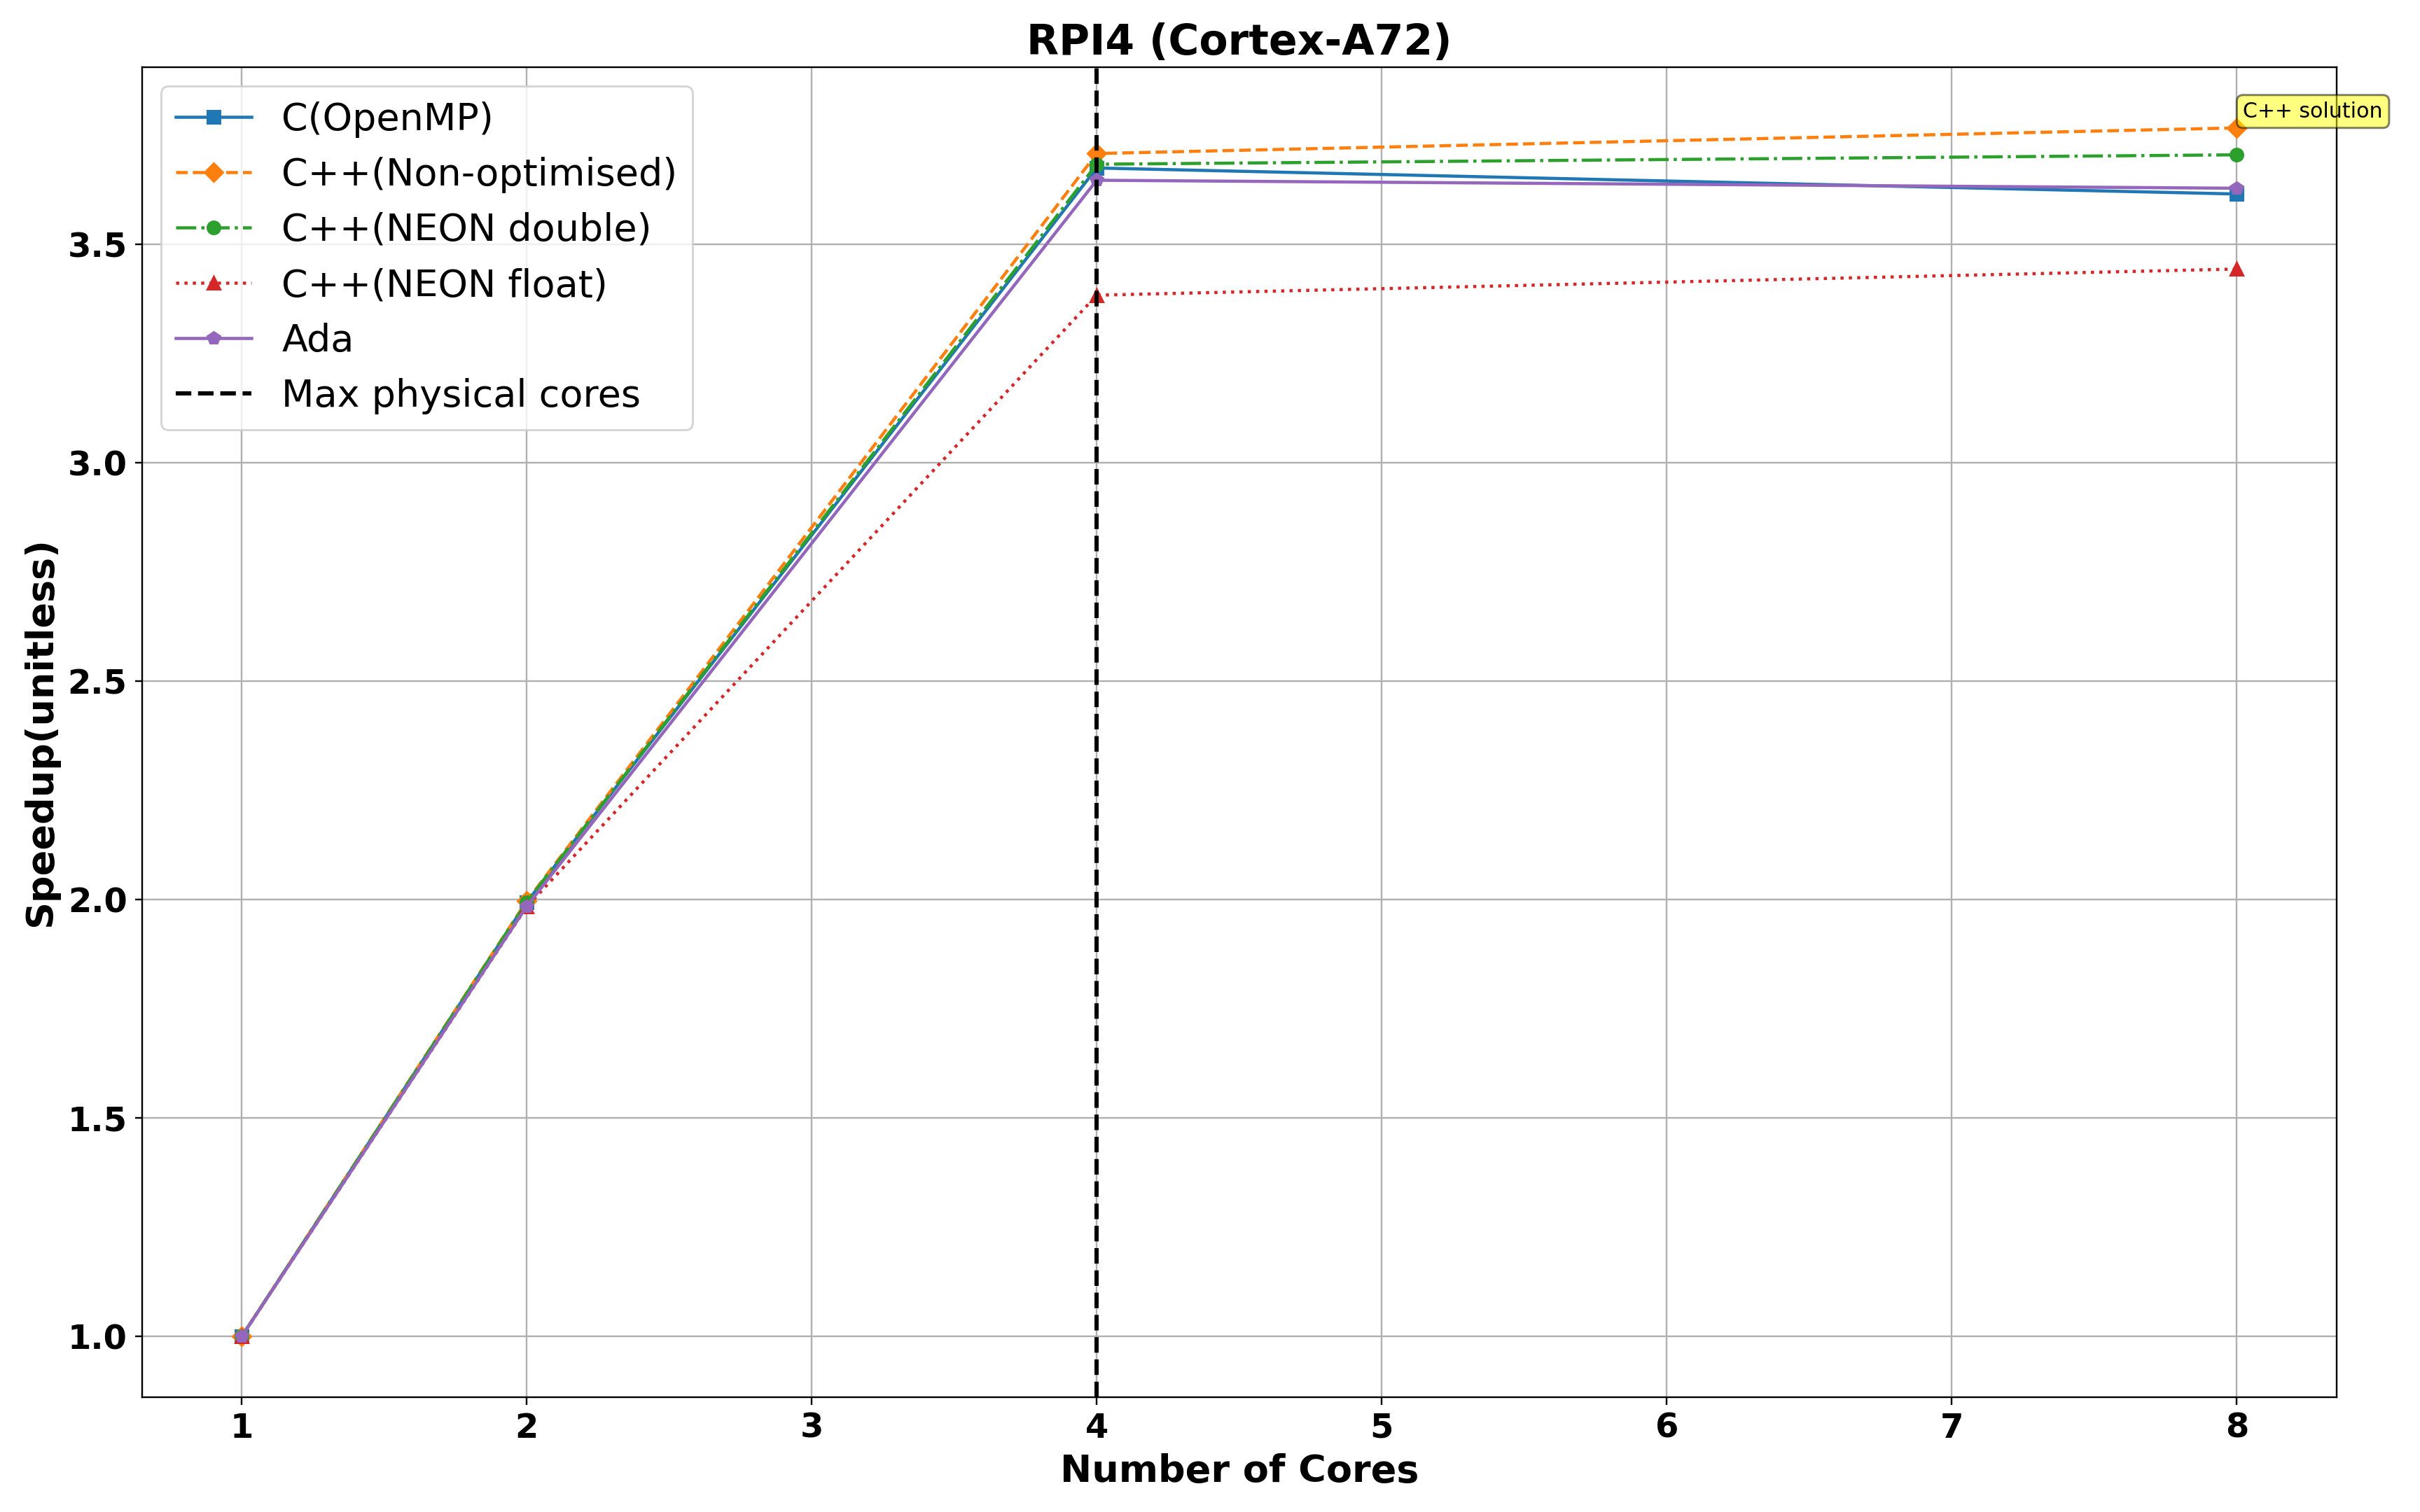
\includegraphics[width=1\textwidth, height=20cm]{~/Documents/Part_D_Modules/Individual_Project/Individual_report/figures/mpbenchmark_rpi4_speedup.png} % Adjust the path and width as needed
	\caption{Speedup plot collected from Raspberry Pi 4 processor. The vertical black line shows the maximum physical cores of the processor. (Higher is better).}
	\label{fig:mpbenchmark_rpi4_speedup_plot} % Use this label to reference the figure
\end{figure}

The decimal precision of using single and double precision floating point \texttt{NEON} instructions on the Raspberry Pi processors is compared in table ~\ref{tab:c++_neon_pi}.

\begin{table}[htbp]
	\centering
	\begin{tabular}{|c|c|c|c|}
		\hline
		\textbf{Programming language/configuration} & \textbf{Decimal value of $\pi$} & \textbf{Run time RPI5(s)} & \textbf{Run time RPI4(s)} \\ \hline
		\texttt{C++}                                                   & 3.1415926535897643 & 0.028356  & 0.115569 \\ \hline
		\texttt{C++/single-precision NEON}                & 3.141531467437744   &  0.016477 & 0.056352 \\ \hline
		\texttt{C++/double-precision NEON}               & 3.14159265358986     & 0.033399  & 0.116423 \\ \hline
		\texttt{C}                                                       &  3.1415926535897643 & 0.031107  & 0.116538\\ \hline 
		\texttt{Ada}                                                    & 3.1415926535897643  & 0.029549  & 0.117536 \\ \hline
	\end{tabular}
	\label{tab:c++_neon_pi}
	\caption{Comparing the decimal precision of the \texttt{NEON} enhanced solutions. RPI5 - Raspberry Pi 5, RPI4- Raspberry Pi 4. Mean benchmark time in seconds collected using maximum cores on the system(4 cores).}
\end{table}

% Talk about the proposed solution's performance in PI5 and PI4. 
% Talk about the speedup
% Talk about NEON solutions and their respective decimal precision.
% Can include the comparision with other solutions in the appendix, like Java and C# and Raspberry Pi 3 

The proposed solution outperformed both the solutions in \texttt{C} and \texttt{Ada} in run time and speedup. On Raspberry Pi 5 a slight reduction in run time(about 4\%) and a notable improvement in speedup was observed. Results on Raspberry Pi 4 were not as impressive as the performance was just about 1\% improvement and a marginal increase in speedup.  Nevertheless, the proposed \texttt{C++} outperformed the original solutions in terms of run time and speedup on both of the Raspberry Pi devices albeit the improvement was marginal on the Raspberry Pi 4. 

The \texttt{NEON} enhanced solutions using single point precision produced over 40\% reduction in time at the cost of a lower speedup across threads, and a reduced decimal precision of 4 decimal places. 


% Round up results and discuss and further research/propositions 
